\section{Bidirectional RNNs}
\begin{frame}{}
  \LARGE RNN : \textbf{Bidirectional RNNs}
\end{frame}

\begin{frame}{Bidirectional RNNs}
  \begin{itemize}
    \item A standard RNN reads left to right: $h_t$ summarizes only the past $x_1, \dots, x_t$.
    \item Many tasks need context from both sides. In ``The bank of the river'', the meaning of ``bank'' depends on words that come later.
    \item A \textbf{bidirectional RNN} (Schuster and Paliwal, 1997) runs two RNNs over the sequence: a forward RNN producing $\overrightarrow{h}_t$ and a backward RNN producing $\overleftarrow{h}_t$.
    \item The representation of each position is the concatenation $h_t = [\overrightarrow{h}_t; \overleftarrow{h}_t]$: past and future context at every step.
  \end{itemize}

  \vspace{0.5em}
  \centering
  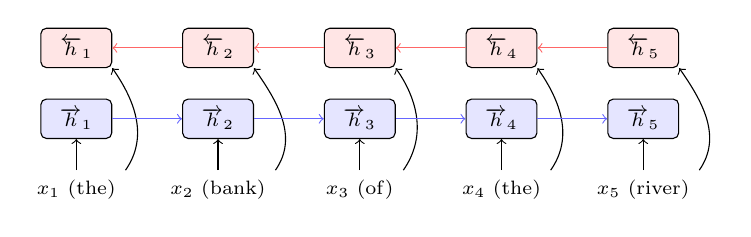
\begin{tikzpicture}[node distance=0.9cm, every node/.style={font=\scriptsize}]
    \foreach \i/\w in {1/the, 2/bank, 3/of, 4/the, 5/river} {
      \node (x\i) at (1.8*\i, 0) {$x_{\i}$ (\w)};
      \node[draw, rounded corners=2pt, minimum width=0.9cm, minimum height=0.5cm, fill=blue!10] (f\i) at (1.8*\i, 0.9) {$\overrightarrow{h}_{\i}$};
      \node[draw, rounded corners=2pt, minimum width=0.9cm, minimum height=0.5cm, fill=red!10] (b\i) at (1.8*\i, 1.8) {$\overleftarrow{h}_{\i}$};
      \draw[->] (x\i) -- (f\i);
      \draw[->] (x\i.north east) to[out=55, in=-55] (b\i.south east);
    }
    \foreach \i/\j in {1/2, 2/3, 3/4, 4/5} {
      \draw[->, blue!60] (f\i) -- (f\j);
      \draw[<-, red!60] (b\i) -- (b\j);
    }
  \end{tikzpicture}
\end{frame}

\begin{frame}{Where Bidirectionality Works, and Where It Cannot}
  \begin{itemize}
    \item \textbf{Works for encoding:} the full input is available before any output is produced.
    \begin{itemize}
      \item Part-of-speech tagging, named entity recognition, sequence classification.
      \item BiLSTMs were the standard sentence encoder before transformers.
    \end{itemize}
    \item \textbf{Does not work for generation:} when producing text token by token, the future does not exist yet, so the backward RNN has nothing to read. Decoders stay unidirectional.
    \item This encoder/decoder split carries into modern models: bidirectional encoders and left-to-right decoders.
  \end{itemize}
\end{frame}
